% ============================================================
% f2012_jiangsu_q21a_circle.tex
% 2012 江苏卷第 21A 题 圆 O 的直径 AB
% D、E 在圆上位于 AB 异侧，BD 延长至 C 且 BD=DC
% 连接 AC、AE、DE（TikZ 矢量重绘）
% ============================================================
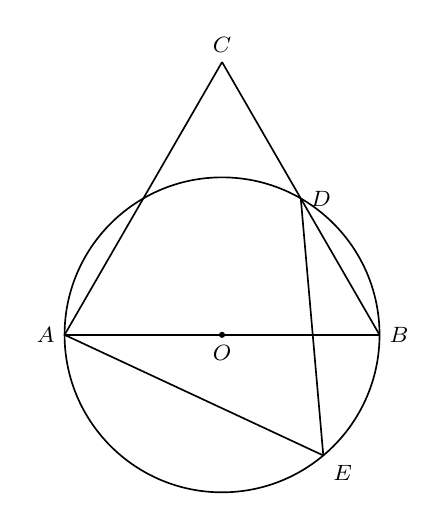
\begin{tikzpicture}[x=1cm, y=1cm, line width=0.6pt, font=\footnotesize]

  \coordinate (O)  at (0,0);
  \coordinate (A)  at (-2,0);
  \coordinate (B)  at (2,0);
  \coordinate (D)  at (1.00,1.732);
  \coordinate (C)  at (0,3.464);
  \coordinate (E)  at (1.286,-1.532);

  % ---------- 圆与直径 ----------
  \draw (0,0) circle (2);
  \draw (A) -- (B);

  % ---------- 题设线段 ----------
  \draw (B) -- (D) -- (C);
  \draw (A) -- (C);
  \draw (A) -- (E);
  \draw (D) -- (E);

  % ---------- 点与标注 ----------
  \fill (O) circle (1.1pt);
  \node[below]       at (O) {$O$};
  \node[left]        at (A) {$A$};
  \node[right]       at (B) {$B$};
  \node[right]       at (D) {$D$};
  \node[above]       at (C) {$C$};
  \node[below right] at (E) {$E$};

\end{tikzpicture}
